% !TeX root = hw8-answers.tex

\chead{\textbf{Exercises week 8}}
\begin{document}
\flushleft\textbf{Topic: Do-calculus and the backdoor criterion}
\section{An intuitive sufficient condition for the backdoor criterion}

In this part of the exercise, we want to gain a more intuitive understanding of the backdoor criterion. 
    Let $G^{+} = (V, U, E^{+})$ be a DAG with $J = \emptyset$, and let $A, B, C \subseteq V$ be pairwise disjoint subsets. 
    The backdoor criterion for identifying causal effects from $B$ to $A$ reads:
    \begin{align*}
     i & )  \quad   C    \Perp^d_{G_{\text{do}(I_B)}} I_B   \\
   ii & )  \quad    A    \Perp^d_{G_{\text{do}(I_B)}} I_B \mid B \cup C
    \end{align*}
    Now, we define a \emph{backdoor walk} from A to B to be any walk which starts in a node in $A$ and ends in a node in $B$ and whose last arrow is of the form $v \rightarrow b$ (instead of $v \leftarrow b$), i.e., it enters $B$ ``from the backdoor''.
    Now consider the following two alternative conditions:
    \begin{align*}
    i' & ) \quad   C \cap \text{Desc}^G(B) = \emptyset \\
  ii' & ) \quad   \text{All backdoor walks from A to B are $d$--blocked by $C$} 
    \end{align*}
    Do the following exercises:
    \begin{enumerate}
\item Prove that i) is equivalent to i'), i.e.: i) implies i') and i') implies i).  \textbf{(1pt)} 
      \item Prove that ii') implies ii).  \textbf{(1pt)} 
\item Show that ii) does not in general imply ii'), i.e.: construct an example for a DAG $G^+$ and disjoint $A, B, C \subseteq V$ such that ii) holds, but ii') does not. \textbf{(1pt)} 
      \end{enumerate}
  This exercise shows that in order to test if the backdoor rule is applicable, you can first see if the more intuitive conditions i') and ii') hold.
      However, these conditions are only \emph{sufficient}, but not \emph{necessary} for the backdoor criterion to be applicable.
Thus, if i') holds, and ii') does not hold, you still have the chance that ii) holds and that adjustment is possible.


    \begin{gradedsolution}
      We show all implications by contraposition.
      \begin{enumerate}
	\item We show both implications separately: 
	  \begin{itemize}
	\item $\neg i \Rightarrow \neg i':$ Assume $C \not\perp^d_{G_{\text{do}(I_B)}} I_B$. 
	  This means that there is a walk $\pi$ from a node $I_b$ with $b \in B$ to a node $c \in C$ which is d-open by $\emptyset$.
	  Consequently, $\pi$ cannot contain any collider. 
	  Note that $I_b$ has only one outgoing arrow to $b$ and no ingoing arrows, so the first edge in $\pi$ needs to be of the form $I_b \to b$.
	  Since there is no collider, by induction each arrow in $\pi$ is of the form $v_i \rightarrow v_{i+1}$.
	  Consequently, $\pi$ is directed. 
	  Cutting off $I_b$, we obtain a directed walk from $b$ to $c$, proving $C \cap \text{Desc}^G(B) \neq \emptyset$.
	\item $\neg i' \Rightarrow \neg i$: We basically do each step in reverse.
	  $C \cap \text{Desc}^G(B) \neq \emptyset$ gives a directed walk from some $b \in B$ to some $c \in C$.
	  Adding the edge $I_b \to b$ at the left, we obtain a non-blocked walk from $C$ to $I_B$, showing $C \not\perp^d_{G_{\text{do}(I_B)}} I_B$.
	\end{itemize}
	\item $\neg ii \Rightarrow \neg ii'$: Assume $A \not\perp^d_{G_{\text{do}(I_B)}} I_B | B \cup C$. 
	  Thus, there is a walk $\pi$ from some $a \in A$ to $I_b$ for some $b \in B$ which is d-open by $B \cup C$.
	  The last edge of $\pi$ is of the form $b \leftarrow I_b$ by definition of $G_{\text{do}(I_B)}$.
	  The edge before that then must be of the form $v \rightarrow b$ (instead of $v \leftarrow b$), for some $v \in V \cup U$ since otherwise $\pi$ would be blocked by $b \in B \subseteq B \cup C$, a contradiction.
	  Now consider the walk $\pi'$ from $a$ to $b$ constructed from $\pi$ by just removing the last edge $b \leftarrow I_b$.
	  It is a backdoor-walk since it ends with $v \rightarrow b$.
	  Now, assume that $\pi$ was actually chosen to have the smallest length possible. 
	  Then, none of the intermediate nodes can be in $B$, since otherwise by the openness that intermediate node would need to be a collider and we could construct a shorter walk to $I_B$.
	  Consequently, $\pi'$ is not only d-open by $C \cup B$, but even d-open by $C$ (reason: colliders must have their middle node in $C \cup B$, and since it cannot be in $B$, it must then be in $C$!).
	  Thus, there is a backdoor walk (namely $\pi'$) from $A$ to $B$ which is d-open by $C$, i.e. we proved $\neg ii'$.
	\item A counterexample is given by the following graph, with $A = \{a\}$, $B = \{b_1, b_2\}$, and $C = \emptyset$: 
\begin{figure}[ht]
  \centering
  \begin{tikzpicture}[scale=1, transform shape]
      \tikzstyle{every node} = [draw,shape=circle,color=blue];
      \node (A) at (2, 0) {$a$};
      \node (B) at (4, 0) {$b_1$};
      \node (X) at (6, 0) {$b_2$};
      \tikzstyle{every node} = [draw,shape=rectangle, color=teal];
      \node (I) at (4, -2) {$I_{b_2}$};
      \node (J) at (8, 0) {$I_{b_2}$};
     \draw[-{Latex[length=3mm, width=2mm]}, color=blue] (B) to (A);
     \draw[-{Latex[length=3mm, width=2mm]}, color=blue] (B) to (X);
     \draw[-{Latex[length=3mm, width=2mm]}, color=teal] (J) to (X);
     \draw[-{Latex[length=3mm, width=2mm]}, color=teal] (I) to (B);
  \end{tikzpicture}
  \label{fig:cadmg}
\end{figure}

	%\item $\neg ii' \Rightarrow \neg ii:$ We again do everything in reverse: 
	%  For a backdoor-walk $\pi'$ from $a \in A$ to $b \in B$ d-open by $C$ chosen to be of minimal length, add the edge $b \leftarrow I_b$ at the end, obtaining a path $\pi$.
	%  Since $\pi'$ is a backdoor walk, it ends with $v \rightarrow b$ for some $v \in V \cup U$, meaning $\pi$ ends with the collider $v \rightarrow b \leftarrow I_b$.
	%  The minimal length assumption guarantees that no intermediate nodes can be in $B$.
	%  Consequently, all non-colliders in $\pi$ are not in $B$, but also not in $C$ since $\pi'$ was chosen d-open by C.
	%  I.e., all non-colliders are not in $B \cup C$.
	%  All intermediate colliders are in $C$ due to the d-openness of $\pi'$ by $C$, and since $C \subseteq B \cup C$, they are even in $B \cup C$.
	%  Finally, the collider $v \rightarrow b \leftarrow I_b$ at the end is in $B \subseteq B \cup C$, as we discussed before.
	%  Overall, we found a walk from $a \in A$ to $I_b \in I_B$ which is d-open by $B \cup C$, proving $\neg ii$.
	\end{enumerate}

    \end{gradedsolution}

    \section{The Simpson's Paradox}

\begin{enumerate}
  \item You are investigating the effectiveness of a drug against a deadly disease.
You are given access to data collected by health insurance companies about
their customers. You divide the diseased customers into two groups: those 
that took the drug, and those that didn't take the drug. 
Some of the customers
recovered, others unfortunately didn't recover. The reasons why some patients
were treated and others were not, are unknown to you. 
You find the following numbers:\\
\vspace{20pt}
\centerline{\begin{tabular}{l|cc|c|c}
 & Recovery & No recovery & Total & Recovery rate \\
\hline
Drug    & 20 & 20 & 40 & \dots\% \\
No drug & 16 & 24 & 40 & \dots\% \\
\hline
Total   & 36 & 44 & 80 & \\
\end{tabular}}

\begin{enumerate}[label=\alph*)]
\item Calculate the recovery rates (in \%) for both groups (``drug'' and ``no drug'').  \textbf{(1/5pts)}

\item If you were diseased, would you take the drug, or not?  \textbf{(1/5pts)}

\end{enumerate}


Upon closer inspection of the data, you notice something peculiar when you group patients according to gender:\\

\vspace{20pt}
\centerline{\begin{tabular}{l|cc|c|c}
\textbf{Males} & Recovery & No recovery & Total & Recovery rate \\
\hline
Drug    & 18 & 12 & 30 & \dots\% \\
No drug &  7 &  3 & 10 & \dots\% \\
\hline
Total   & 25 & 15 & 40 & \\
\end{tabular}}
\medskip
\centerline{\begin{tabular}{l|cc|c|c}
\textbf{Females} & Recovery & No recovery & Total & Recovery rate \\
\hline
Drug    &  2 &  8 & 10 & \dots\% \\
No drug &  9 & 21 & 30 & \dots\% \\
\hline
Total   & 11 & 29 & 40 & \\
\end{tabular}}

\begin{enumerate}[resume*]
  \item Calculate the recovery rates (in \%) for both groups (``drug'' and ``no drug''), for each subpopulation (males and females) separately.  \textbf{(1/5pts)}


  \item In light of these numbers, would you take the drug if you were diseased, or not?  \textbf{(1/5pts)}


  \item What would be your advice to a diseased patient with unknown gender?  \textbf{(1/5pts)}
\end{enumerate}

This phenomenon is known as ``Simpson's paradox''.
A lot has been written about this paradox, but it dissolves once you recognize that you should not make the mistake of interpreting correlations as causations, as we'll see in the next part of the exercise.


 
  \item 
We will make use of causal reasoning with IL-CBNs to resolve Simpson's paradox.

\begin{figure}[h]
  \centerline{%
    \begin{tikzpicture}
      \begin{scope}
        \node[var] (M) at (0,1) {$M$};
        \node[var] (D) at (-1,0) {$D$};
        \node[var] (R) at (1,0) {$R$};
        \draw[arr] (M)--(D);
        \draw[arr] (M)--(R);
        \draw[arr] (D)--(R);
        \node at (-2,1) {(i)};
      \end{scope}
      \begin{scope}[xshift=6cm]
        \node[var] (M) at (0,1) {$M$};
        \node[var] (D) at (-1,0) {$D$};
        \node[var] (R) at (1,0) {$R$};
        \draw[arr] (D)--(M);
        \draw[arr] (M)--(R);
        \draw[arr] (D)--(R);
        \node at (-2,1) {(ii)};
      \end{scope}
      \begin{scope}[xshift=12cm]
        \node[var] (M) at (0,1) {$M$};
        \node[var] (D) at (-1,0) {$D$};
        \node[var] (R) at (1,0) {$R$};
        \node[varh] (L1) at (-1,2) {$L_1$};
        \node[varh] (L2) at (1,2) {$L_2$};
        \draw[arr] (D)--(R);
        \draw[arrh] (L1)--(M);
        \draw[arrh] (L2)--(R);
        \draw[arrh] (L1)--(D);
        \draw[arrh] (L2)--(M);
        \node at (-2,1) {(iii)};
      \end{scope}
    \end{tikzpicture}
  }
\caption{Different hypothetical causal graphs, where $R$ stands for \emph{Recovery}, $D$ for taking the \emph{Drug}, and $M$ has different interpretations in cases (i), (ii) and (iii).\label{fig:Simpson}}
\end{figure}

Suppose you believe that an IL-CBN with causal graph as in Figure \ref{fig:Simpson}(i) applies, where $M$ denotes gender of the patient (male/female).

\begin{enumerate}[label=\alph*)]
\item \label{Simpson_1} Apply the back-door criterion to obtain a formula that expresses $P(R \given \text{do}(D))$ in terms of observable quantities (i.e., in terms of marginal or conditional distributions where the \emph{do}-operator does not appear).  \textbf{(1/5pts)}

%In this case, we need to adjust for $\{M\}$ when calculating $p(R \given \text{do}(D))$:
%      $$p(R \given \text{do}(D)) = \sum_{M} p(R \given D, M) p(M) \ne p(R \given D)$$


\item Is $P(R \given \text{do}(D)) = P(R \given D)$ in this case?  \textbf{(1/5pts)}


\item What would be your advice for a patient with unknown gender?  \textbf{(1/5pts)}

\end{enumerate}

Now suppose that instead, you believe that an IL-CBN with causal graph as in Figure \ref{fig:Simpson}(ii) applies. Intuitively, this would be quite unlikely, as we
know that most drugs don't change gender, but we could have used a slightly different story where the variable $M$ has a different interpretation
(for example, ``blood pressure''), and then this causal structure would also be a plausible one.

\begin{enumerate}[resume*]
  \item Again, use the back-door criterion to express $P(R \given \text{do}(D))$ in terms of observable quantities.  \textbf{(1/5pts)}


  \item Is $P(R \given \text{do}(D)) = P(R \given D)$ in this case?  \textbf{(1/5pts)}


\item \label{Simpson_2} What would be your advice for a patient with unknown $M$ (say, blood pressure) in this case?  \textbf{(1/5pts)}

\end{enumerate}

Finally, suppose that you believe that the IL-CBN has the causal graph of Figure \ref{fig:Simpson}(iii), with two
latent variables $L_1,L_2$.

\begin{enumerate}[resume*]
  \item Invent an interpretation of $M$ and the two latent variables $L_1,L_2$ yourself that could match the causal model depicted in Figure \ref{fig:Simpson}(iii).  \textbf{(1/5pts)}


\item Express $P(R \given \text{do}(D))$ in terms of \emph{observable} quantities.  \textbf{(1/5pts)}


\item Is $P(R \given \text{do}(D)) = P(R \given D)$ in this case?  \textbf{(1/5pts)}


\item Again, what would be your advice for a patient with unknown $M$ in this case?  \textbf{(1/5pts)}

\end{enumerate}

Conclusion: whether or not you should prescribe the drug depends on which causal model you believe to apply to this situation. 
The fact that different causal models will lead to different conclusions should not be paradoxical, it is another illustration that
``correlation does not imply causation''.

 
\end{enumerate}

\begin{gradedsolution}
  \begin{enumerate}
    \item
      \begin{enumerate}[label=\alph*)]
	\item Drug: 50\%; No drug: 40\%. 
	\item The data provided does not contain enough information to decide rationally (at first sight, one might think that taking the drug is advantageous).
	\item Males: Drug 60\%; No drug 70\%.\\
Females: Drug 20\%; No drug 30\%. 
	\item  The data provided does not contain enough information to decide rationally (at first sight, one might think that taking the drug is disadvantageous for both males and females).
	\item The data provided does not contain enough information to decide rationally.
	\end{enumerate}
    \item
      \begin{enumerate}[label=\alph*)]
	\item We are looking for a subset of covariates that satisfies the assumptions of the back-door criterion. There are only two possible
subsets of covariates in this simple case: $\emptyset$ and $\{M\}$. According to the back-door criterion, we can adjust for $\{M\}$:
$$p(R \given \text{do}(D)) = p(R \given D, M) \circ p(M).$$
	\item No, for this causal model $p(R \given \text{do}(D)) \ne p(R \given D)$ (except possibly for specifically tuned parameters of the model). Indeed,
note that $p(R \given D) = p(R \given D, M) \circ p(M \given D)$, and for the model in Figure \ref{fig:Simpson}(i), in general $p(M) \ne p(M \given D)$ (because of Bayes' theorem). 
	\item First of all, one should realize that treating the patient is an \emph{intervention}: we are actively setting the random variable $D$ to some value.
Therefore, we are interested in the quantity $p(R \given \text{do}(D))$, and not in $p(R \given D)$ (which lead to the paradox). We can calculate
    $p(R \given \text{do}(D))$ using the adjustment formula in \ref{Simpson_1}. As $p(R|D=1,M) < p(R|D=0,M)$ for both genders, the same will hold for a mixture:
$p(R \given \text{do}(D=1)) < p(R \given \text{do}(D=0))$. So assuming
the causal structure in Figure \ref{fig:Simpson}(i), the advice would be not to take the drug.
	\item Now $M$ is a descendant of $D$, so we cannot use $\{M\}$ for adjustment. There are no back-door paths $D \leftarrow \dots \dots R$, so
$\emptyset$ is sufficient for adjustment:
$$p(R \given \text{do}(D)) = p(R \given D)$$ 
	\item Yes.   
	\item As $p(R \given D=1) > p(R \given D=0)$, this means that now $p(R \given \text{do}(D=1)) > p(R \given \text{do}(D=0))$. So assuming the causal
structure is as in Figure \ref{fig:Simpson}(ii), the advice for (all) patients is to take the drug.
	\item Left to the imagination of the reader.  
	\item $\emptyset$ is sufficient for adjustment according to the back-door criterion, so
$$p(R \given \text{do}(D)) = p(R \given D).$$
	\item Yes.   
	\item Same as in \ref{Simpson_2}: all patients should take the drug.
	\end{enumerate}
    \end{enumerate}
\end{gradedsolution}



\section{Selection bias and the do-calculus}

Selection bias is a problem in the inference of observational and causal relationships.
For example, imagine that you want to measure the effect of some societal intervention on household incomes.
It is known that people are more likely to report their income if it is higher, which can make it hard to estimate the effects of the intervention if people can self-select to report.

Nevertheless, sometimes one can estimate causal effects even in such self-selection scenarios, and in this exercise we go through such an example.\footnote{The example is taken from the paper ``Recovering from Selection Bias in Causal and Statistical Inference'' by Elias Bareinboim et al.}
For this, look at Figure \ref{fig:selection_effect}.

\begin{figure}
  \centering
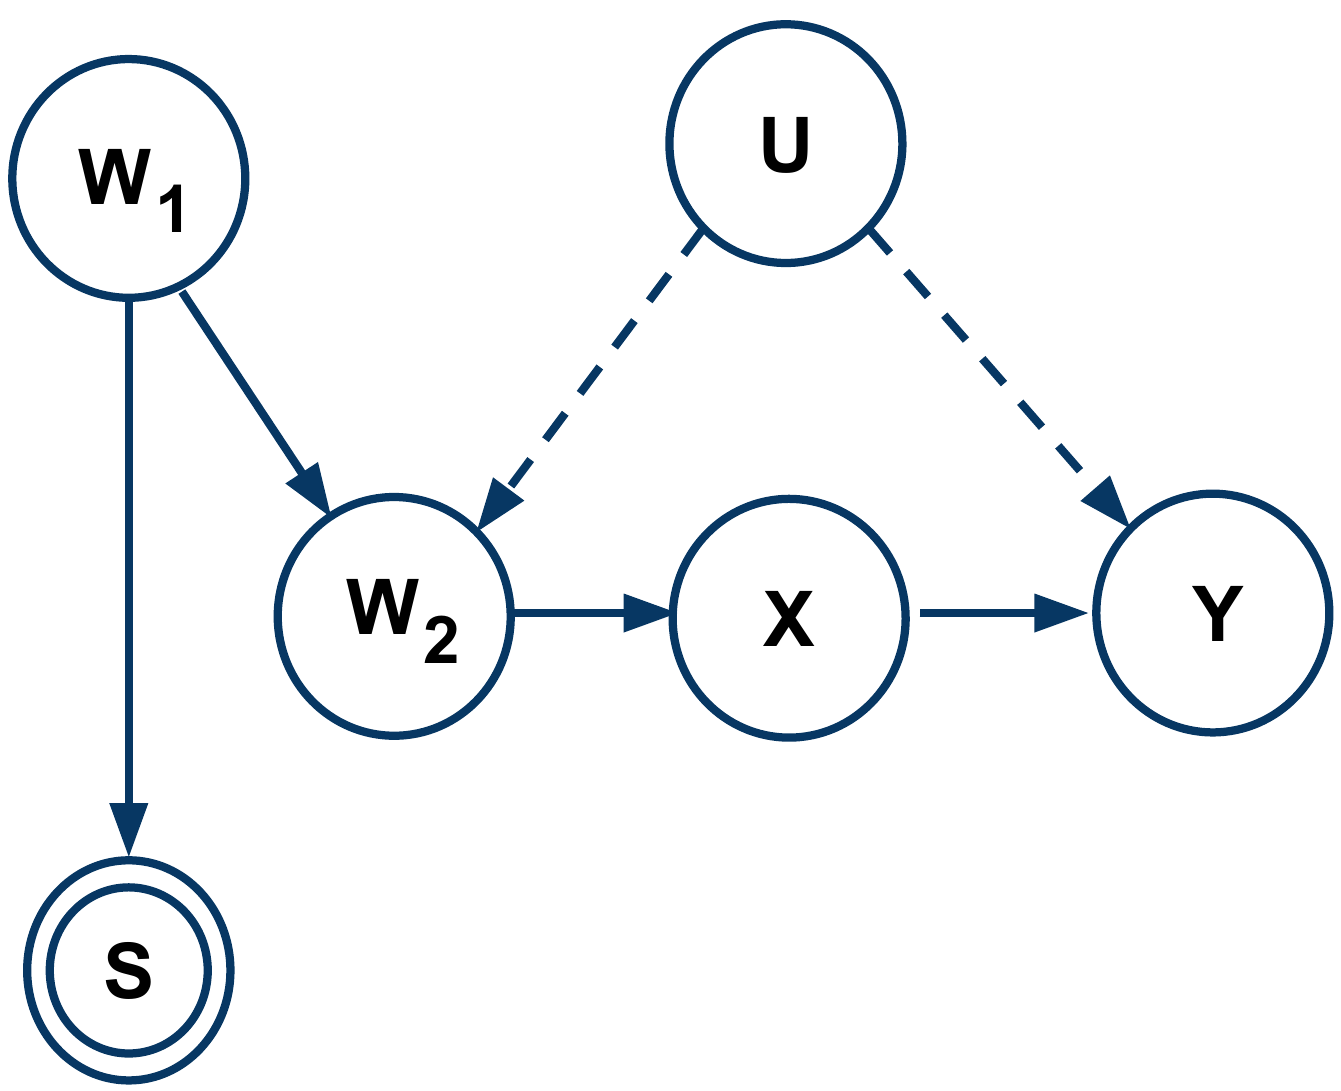
\includegraphics[width=0.6\textwidth]{bareinboim}
\caption{In this causal graph, $U$ is a latent variable and $S$ a selection variable.
The goal is to determine the causal effect of $X$ on $Y$ purely from observational data conditioned on the selection $S = 1$.}
\label{fig:selection_effect}
\end{figure}

$S$ can take two values, $S = 1$ (selected) and $S = -1$ (not selected). 
For convenience, we thereby use the same symbols for the nodes in the causal graph and for the random variables appearing in the corresponding Markov kernels.
You want to determine the causal effect $P(Y | \text{do}(X))$, however, there are three caveats:
\begin{itemize}
  \item You only have observational data and did not perform an intervention, and so you must express this without a do-operation. 
  \item $U$ is latent and not observed, and so it cannot appear in the final formula. 
  \item You only see data in cases where a selection happened ($S = 1$), and so you only have access to an estimation of the conditional probability $P(W_1, W_2, X, Y | S = 1)$ 
  \end{itemize}

  In the following exercises, you will use the do-calculus to show that this does not pose an actual problem:

  \begin{enumerate}
    \item Show that $P(Y | \text{do}(X)) = P(Y | S, \text{do}(X))$.  \textbf{(1pt)} 
    \item Show that $P(Y | S, \text{do}(X)) = P(Y | S, W_2, \text{do}(X)) \circ P(W_2 | S)$.  \textbf{(1pt)} 
    \item Show that  $P(Y | S, W_2, \text{do}(X)) = P(Y | S, W_2, X)$.  \textbf{(1pt)} 
    \item Argue that we have reached our goal.  \textbf{(1pt)} 
    \end{enumerate}

    \begin{gradedsolution}
      \begin{enumerate}
	\item For applying the do-calculus rule for ``insertion/deletion of observation'', we need to check the following separation:
	  \begin{equation*}
	    Y \Perp_{G_{\text{do}(X)}}^{d} S | X.
	  \end{equation*}
	  Paths from $Y$ to the input node $X$ are automatically blocked by $X$.
	  There are two paths from $Y$ to $S$, namely $Y \leftarrow X \leftarrow W_2 \leftarrow W_1 \rightarrow S$, which is invalid since we cut of the parents of $X$, and $Y \leftarrow U \rightarrow W_2 \leftarrow W_1 \rightarrow S$, which is blocked at $W_2$, since this is a collider unequal to $X$.
	  Overall, all paths from $Y$ to $\{X, S\}$ are $d$-blocked by $X$, proving the separation-statement, and subsequently the insertion of observation $P(Y | \text{do}(X)) = P(Y | S, \text{do}(X))$.
	\item We introduce the operator $\text{marg}_{W_2}$, which takes a Markov kernel and marginalizes it over $W_2$.
	  With this, we claim the following equalities:
	  \begin{align*}
	    P(Y | S, \text{do}(X)) & \overset{(1)} = \text{marg}_{W_2} P(Y, W_2 | S, \text{do}(X)) \\
	    & \overset{(2)} = \text{marg}_{W_2}  \left[ P(Y | S, W_2, \text{do}(X)) \otimes P(W_2 | S) \right] \\
	    & \overset{(3)} = P(Y | S, W_2, \text{do}(X)) \circ P(W_2 | S).
	  \end{align*}
	  Step 1 is clear.

	  For step 2, we first use the definition of the conditional Markov kernel to obtain
	  \begin{equation*}
	    P(Y, W_2 | S, \text{do}(X)) = P(Y | S, W_2, \text{do}(X)) \otimes P(W_2 | S, \text{do}(X)).
	  \end{equation*}
	  Thus, we need to show the ``deletion of action'' $P(W_2 | S, \text{do}(X)) = P(W_2 | S)$ to be done.
	  This means we need to show the separation statement
	  \begin{equation*}
	    W_2 \Perp_{G_{\text{do}(I_X)}}^d I_X | S.
	  \end{equation*}
	  The two paths from $W_2$ to $I_X$ are $W_2 \rightarrow X \leftarrow I_X$, which is d-blocked by $S$ due to the collider at $X$, and $W_2 \leftarrow U \rightarrow Y \leftarrow X \leftarrow I_X$, which is now open at $X$, but d-blocked by $S$ at $Y$, since this is a collider.
	  Overall, this was to show.

	  For step 3, one can directly apply Remark 5.2.7 from the lecture notes on the connection between product Markov kernels and compositions of Markov kernels.
	\item For the ``action/observation exchange'' we need to show the following separation:
	  \begin{equation*}
	    Y \Perp_{G_{\text{do}(I_X)}}^d I_X | \{X, S, W_2\}
	  \end{equation*}
	  There are two paths from $Y$ to $I_X$, namely $Y \leftarrow X \leftarrow I_X$, which is blocked by X since this is a non-collider, and $Y \leftarrow U \rightarrow W_2 \rightarrow X \leftarrow I_X$.
	  This second path is open at $X$, since this is an opened collider. However, at $W_2$ we have a blocked non-collider, meaning that overall, this path is also blocked.
	  Overall, this shows the separation-statement, and subsequently we can replace the action by an observation: $P(Y | S, W_2, \text{do}(X)) = P(Y | S, W_2, X) $.
	\item Overall, we have proven the formula 
	  \begin{equation*}
	    P(Y | \text{do}(X)) = P(Y | S, W_2, X) \circ P(W_2 | S).
	  \end{equation*}
	  This means that the right-hand-side does not depend on the selection-variable at all, and we can compute the effect of an intervention on $X$ on the distribution over $Y$ as:
	  \begin{equation*}
	    P(Y | \text{do}(X = x)) = P(Y | S = 1, W_2, X = x) \circ P(W_2 | S = 1).
	  \end{equation*}
	  The right-hand-side is conditioned on $S=1$, does not use a do-operation, and does not make use of the latent-variable $U$, and so we can compute it from the observational distribution $P(W_1, W_2, X, Y | S=1)$ and reached our goal.
	\end{enumerate}
    \end{gradedsolution}

\end{document}
